\documentclass[journal, a4paper]{IEEEtran}

\usepackage{graphicx}
\usepackage{url}
\usepackage{amsmath} 
\usepackage{subcaption}

\begin{document}

	\title{Assignment II\\Neural Networks and Deep Learning}
	\author{Adam Kosiorek}	
	\markboth{Machine Learning for Applications in Computer Vision, Institute of Computer Vision, Technische Universit\'at M\"unchen}{}
	\maketitle
	
	
\section{Objective}
    \PARstart{T}{he} aim of the second assignment was to develop thorough understanding of deep neural networks. Firstly, through literature research and derivation of Backpropagation algorithm for arbitrary activation functions we gained insight into the inner workings of feed-forward neural networks. Secondly, we learned how to use a state-of-the-art open-source neural network package \textit{caffe} \cite{caffe} by classifying given images.

\section{Neural Networks and Deep Learning}
    Neural networks are nothing more than a composition of series of non-linear functions and matrix-matrix products. Yet, due to clever learning algorithms, they can be trained to approximate any function. Before we can teach a network, however, we need a dataset of inputs and ground truth pairs as well as a cost function. The latter quantifies differences between network's output and the ground truth for a given input and is being minimized by the training procedure on the whole dataset. The term ``deep learning'' describes neural networks with hidden layers - the layers between input and output layers. It is believed that deep networks learn feature hierarchies, thus alleviating the need for feature engineering.

\section{Deriving Backpropagation}
    In his book, M.~Nielsen derived the Backpropgation algorithm for the sigmoid activation function $\sigma$ \cite{MLDL}. Here, following the notation, I derive it for an arbitrary function $f$.
    
    Let $\delta_j^L$ be the error of $j^{th}$ output neuron, then:
    \begin{equation}
      \delta_j^L = \frac{\partial C(a^L)}{\partial z_j^L} = \frac{\partial C(a^L)}{\partial a_j^L} \frac{\partial a_j^L}{\partial z_j^L}
    \end{equation}
    
    where:
    
    \begin{equation}
      \frac{\partial a_j^L}{\partial z_j^L} = \frac{\partial f(z^L)}{\partial z_j^L} = f'(z_j^L)
    \end{equation}
    
    and thus:
    
    \begin{equation}
      \delta^L = \nabla C(a^L) \odot f'(z^L)
    \end{equation}
    
    For the previous layer, denoted $l$:
    
    \begin{equation}
    \begin{gathered}
      \delta^l = \frac{\partial C(a^L)}{\partial z^l} = \frac{\partial a^L}{\partial z^l} \nabla C(a^L) = \\ = \frac{\partial z^L}{\partial z^l} (f'(z^L) \odot \nabla C(a^L) ) = \frac{\partial z^L}{\partial z^l} \delta^L = \\ = diag(f'(z^l))(w^L)^T \delta^L = f'(z^l) \odot ((w^L)^T \delta^L)
    \end{gathered}
    \end{equation}
    
    Since relations between any two adjacent layers are the same it holds that:
    
    \begin{equation}
      \delta^l  = f'(z^l) \odot ((w^{l+1})^T \delta^{l+1})
    \end{equation}
    
    The final equations for gradients w.r.t. weights and biases do not depend on the activation function and have the same form as in \cite{MLDL}.    
    		
\section {Classification}
  \textit{caffe} is easy to use. Written in C++ with CUDA acceleration, it is high performance, yet, due to Python and Matlab bindings and configuration-oriented architecture it is user-friendly. After completing \textit{ImageNet classification} Notebook I have written a custom script for the assignment~\cite{code}.
  
  \subsection{Configuration}
    Every neural network in \textit{caffe} needs to be configured before being operational. It needs a deployment configuration file - Google Protocol Buffer file defining the network with free (e.g. non-database) inputs and a trained model. Since we wanted the output class name after classification we also need a synset file with class names and identifiers from ILSVRC2012 \cite{ImageNet}
   
  \subsection{Data Preparation}
    Provided images are 3-channel with various sizes and aspect ratios, while the reference \textit{caffe} model operates on $256\times 256\times 3$ data. Convolutional neural networks are scale invariant but are sensitive to changes in aspect ratio. I have therefore resized each input image to 256 px on the longer size and then padded it with zeros to form a square matrix. Padding with zeros should not affect classification, since zeros do not contribute to convolution results. Moreover, the training data for the ImageNet model had intensity values between 0 and 255 and was preprocessed by subtracting mean value computed on the whole dataset and I preprocessed input images accordingly.
    
  \subsection{Results and Discussion}
    Figure \ref{fig:imgs} depicts images given for classification and table \ref{tab:results} shows results. Only images (f) and (g) were classified correctly, as might be suggested by high classification probability and low entropy. Images (e) and (h) can be seen as similar to their predicted categories with lower classification probability and higher entropy. All other images have very low probability and high entropy, suggesting that the classifier is wrong. It seems that classification probability and entropy can be good measures of prediction credibility. According to expectations, the lower the probability (the wider it is spread), the higher the entropy.


  \begin{figure}[h]
    \begin{subfigure}{.25\textwidth}
      \centering
      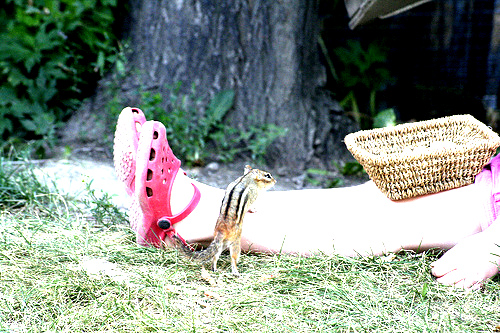
\includegraphics[width=.8\linewidth]{../data/IMG_1}
      \caption{}
      \label{fig:a}
    \end{subfigure}%
    \begin{subfigure}{.25\textwidth}
      \centering
      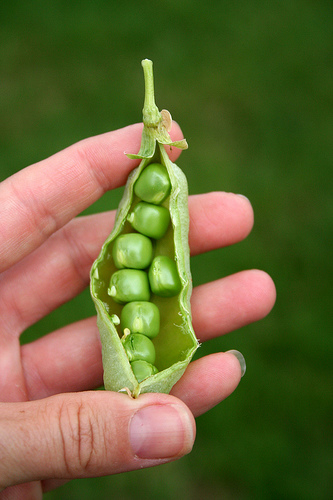
\includegraphics[width=.8\linewidth]{../data/IMG_2}
      \caption{}
      \label{fig:b}
    \end{subfigure}

    \begin{subfigure}{.25\textwidth}
      \centering
      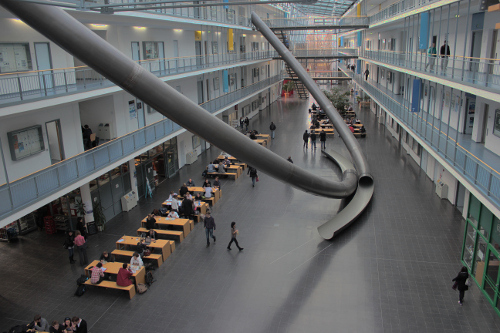
\includegraphics[width=.8\linewidth]{../data/IMG_3}
      \caption{}
      \label{fig:c}
    \end{subfigure}%
    \begin{subfigure}{.25\textwidth}
      \centering
      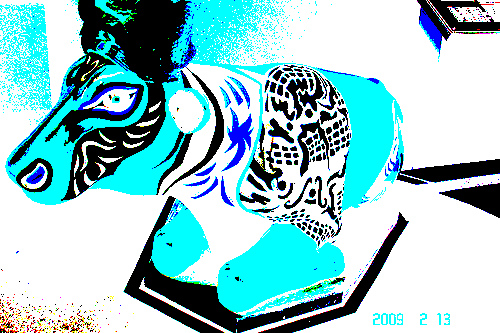
\includegraphics[width=.8\linewidth]{../data/IMG_4}
      \caption{}
      \label{fig:d}
    \end{subfigure}

    \begin{subfigure}{.25\textwidth}
      \centering
      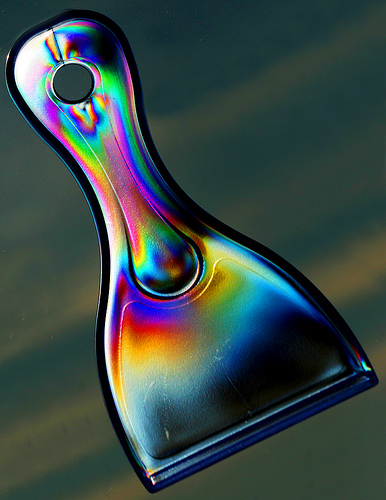
\includegraphics[width=.8\linewidth]{../data/IMG_5}
      \caption{}
      \label{fig:e}
    \end{subfigure}%
    \begin{subfigure}{.25\textwidth}
      \centering
      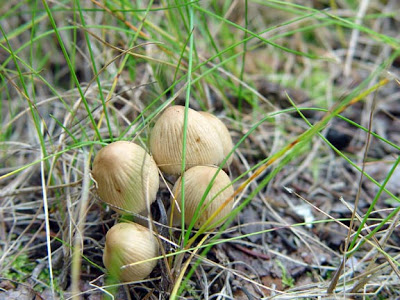
\includegraphics[width=.8\linewidth]{../data/IMG_6}
      \caption{}
      \label{fig:f}
    \end{subfigure}

    \begin{subfigure}{.25\textwidth}
      \centering
      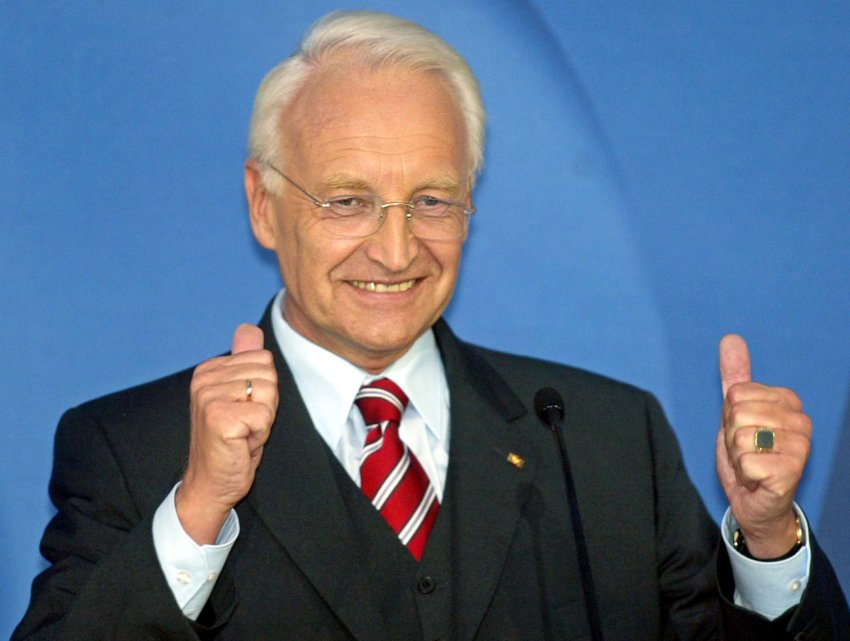
\includegraphics[width=.8\linewidth]{../data/IMG_7}
      \caption{}
      \label{fig:g}
    \end{subfigure}%
    \begin{subfigure}{.25\textwidth}
      \centering
      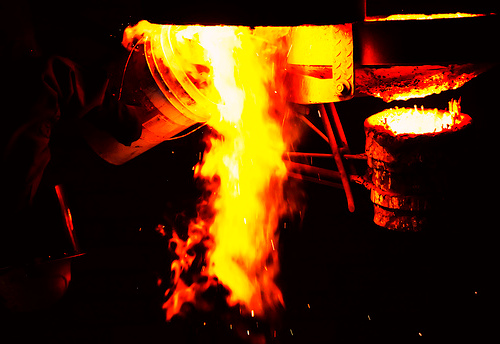
\includegraphics[width=.8\linewidth]{../data/IMG_8}
      \caption{}
      \label{fig:h}
    \end{subfigure}

    \caption{Images for Classification.}
    \label{fig:imgs}
  \end{figure}


  \begin{table}[h]
    \begin{center}
    \caption{Classification Results}
    \label{tab:results}
    \begin{tabular}{c|c|c|c|c}
      \# & \#class  & class name  & probability & entropy \\ \hline
      a & 428 & barrow, garden cart, lawn cart, \ldots & 0.07 & 5.22\\ \hline
      b & 311 & grasshopper, hopper & 0.14 & 3.72\\ \hline
      c & 403 & aircraft carrier, carrier, flattop, \ldots & 0.13 & 4.67\\ \hline
      d & 620 & laptop, laptop computer & 0.12 & 4.63\\ \hline
      e & 673 & mouse, computer mouse & 0.41 & 2.75\\ \hline
      f & 947 & mushroom & 0.76 & 1.17\\ \hline
      g & 834 & suit, suit of clothes & 0.62 & 1.09\\ \hline
      h & 980 & volcano & 0.36 & 3.32
    \end{tabular}
    \end{center}
  \end{table}


\begin{thebibliography}{5}

	\bibitem{code}
	Assignment Code: \url{https://github.com/akosiorek/CSE/tree/master/MLCV/ex2/}
	
	\bibitem{MLDL} % Web document
	M.~A.~Nielsen, ``Neural Networks and Deep Learning'', Determination Press, 2015
	\url{http://neuralnetworksanddeeplearning.com}.
	
	\bibitem{caffe}
	Y.~Jia, E.~Shelhamer, J.~Donahue, S.~Karayev, J.~Long, R.~Girshick, S.~Guadarrama and T.~Darrell, ``Caffe: Convolutional Architecture for Fast Feature Embedding.'' arXiv preprint arXiv:1408.5093, 2014.
	
	\bibitem{ImageNet}
	\url{http://image-net.org/challenges/LSVRC/2012/index}

\end{thebibliography}

% Your document ends here!
\end{document}
